\documentclass[]{article}

\usepackage[]{geometry}
\geometry{
  top=1in,            % <-- you want to adjust this
  inner=1in,
  outer=1in,
  bottom=1in,
  headheight=3ex,       % <-- and this
  headsep=2ex,          % <-- and this
}
\usepackage[T1]{fontenc}
\usepackage{cmbright}
\usepackage{mathtools}
\usepackage{algorithmic}
\usepackage{fancyhdr}
\usepackage{amssymb}
\usepackage{multicol}
\usepackage{parskip}
\usepackage{titling}
\usepackage{fancyvrb}
\pretitle{\begin{flushleft}\LARGE\sffamily}
\posttitle{\par\end{flushleft}\vskip 0.5em}
\preauthor{\begin{flushleft}}
\postauthor{\par\end{flushleft}}
\predate{\begin{flushleft}\scshape}
\postdate{\par\end{flushleft}}
\setlength{\droptitle}{-20pt}
\setlength{\headheight}{15.2pt}
\pagestyle{fancy}

\setcounter{secnumdepth}{1}

\fancyhf{}
\renewcommand{\headrulewidth}{0pt} % remove line at top
\lhead{\fancyplain{}{CS 4780 A3}}
\rhead{\fancyplain{}{Justin Cheng \emph{jc882}, Sunling Selena Yang \emph{sy483}}}
\rfoot{\fancyplain{}{\thepage}}

\begin{document}

\title{CS 4780 Assignment 3}
\author{Justin Cheng \emph{jc882} and Sunling Selena Yang \emph{sy483}}
\date{\today}
\maketitle

\hrule
\vskip 1em

\section{Perceptron and SVM}
\subsection{a.}
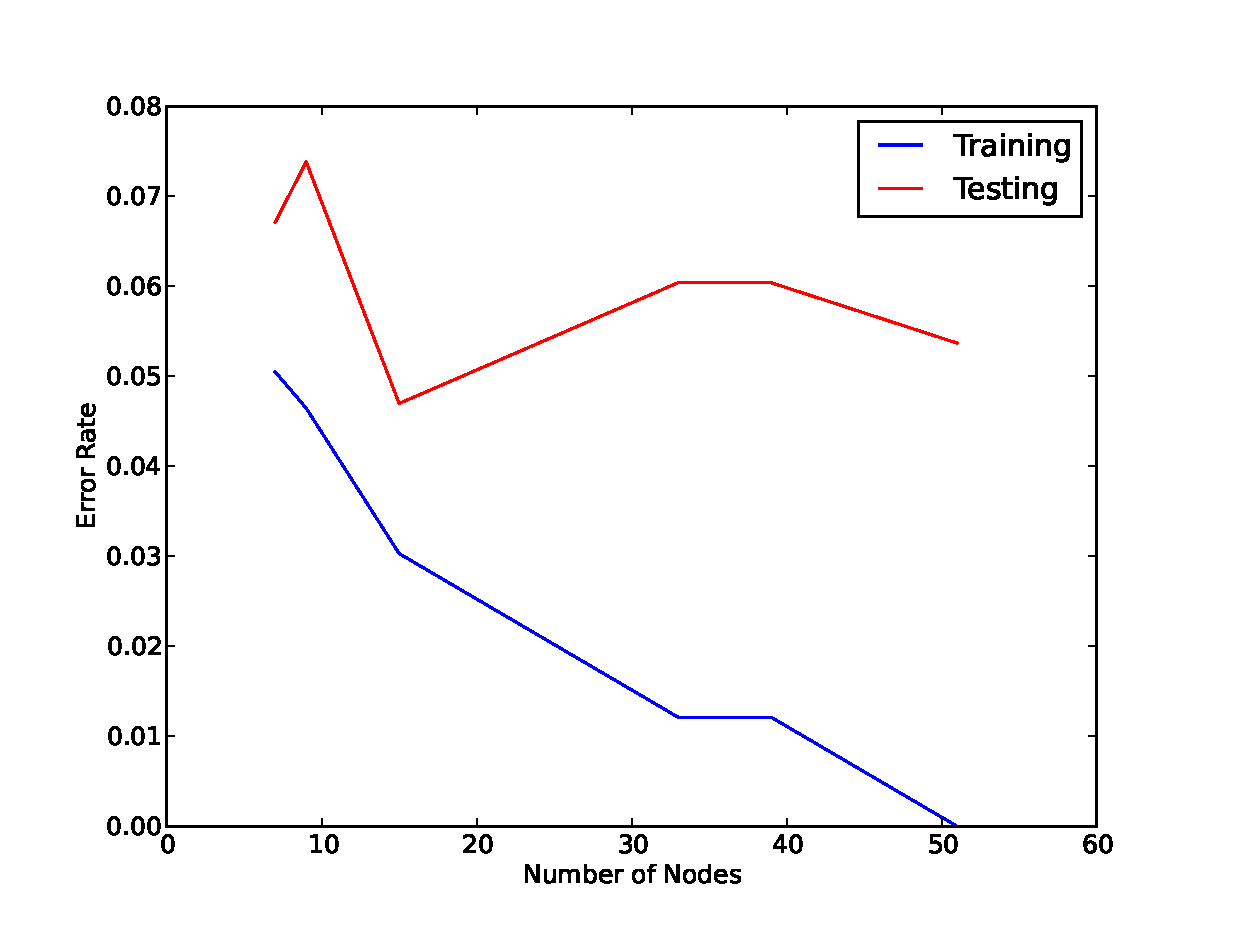
\includegraphics[scale=0.5]{data/images/part_a.eps}

The training error decreases dramatically after the first few iterations, although it is not strictly decreasing. However, after the 15th iteration the training error is 0, meaning that a separating hyperplane was learnt.

The validation error fluctuates wildly for the first few iterations, but then stabilizes at about 0.227.

This does appear to confirm the fact that the Perceptron algorithm converges after a finite number of iterations, and slightly overfits when iterated too many times.

The perceptron should prefer a lower learning rate for improved accuracy, though over a longer number of iterations, since increasing the learning rate speeds up convergence around the true separating hyperplane.. If the learning rate is too high, over-correction is likely to occur and you might end up oscillating around the true separating hyperplane.

Prefer to use the primal algorithm, since computation in each iteration requires using the whole matrix of training examples and storing the alpha values for each example, rather than a single $1\times n$ dimensional matrix if $n$ is the number of unique features. Either algorithm should be equally correct. However, the dual algorithm does provide us with additional expressive power since we can see how important certain examples are by examining their corresponding $\alpha$ values.

\subsection{b.}
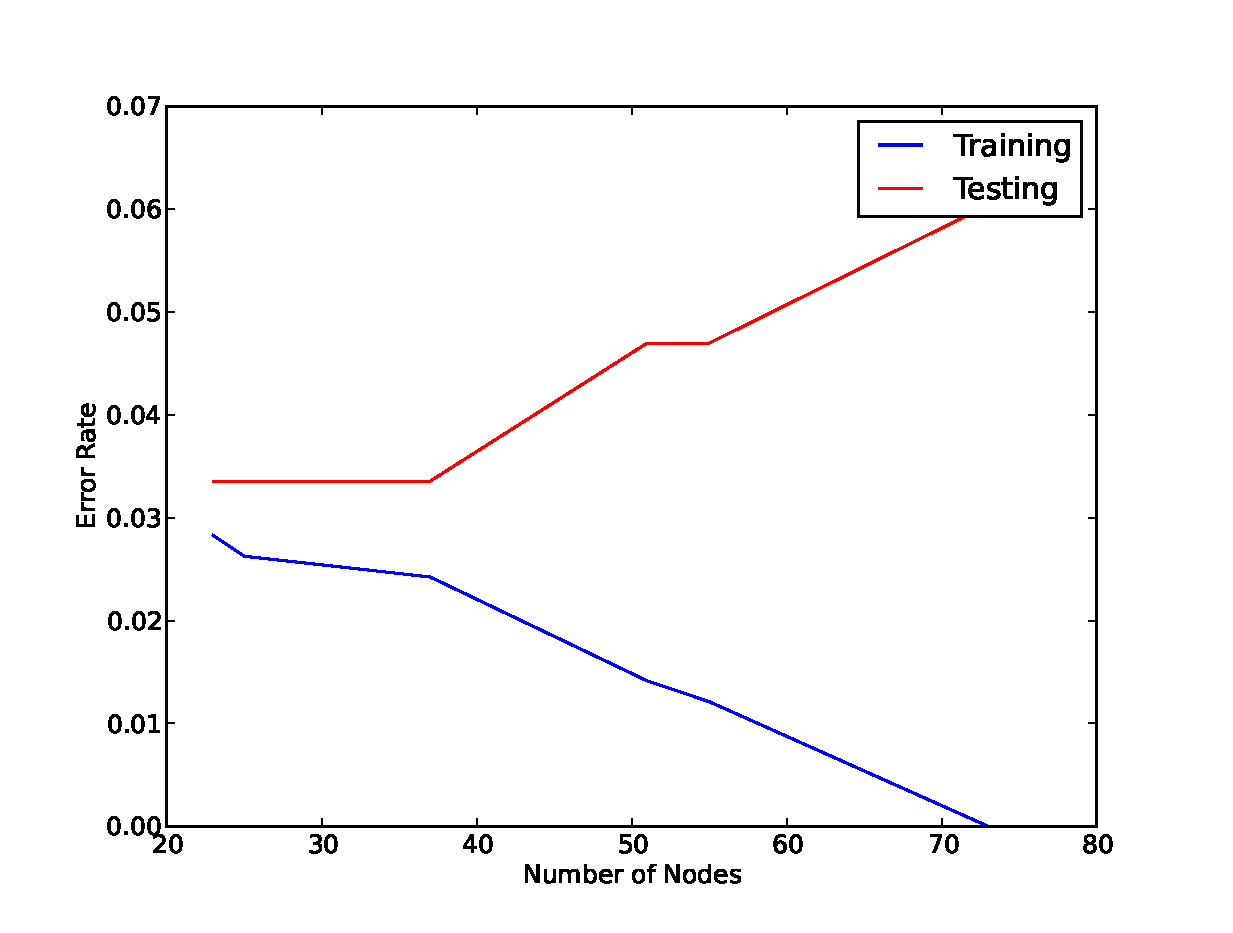
\includegraphics[scale=0.5]{data/images/part_b.eps}

The smallest validation error rate is achieved at $C = 8$. This error rate, $0.205$, is superior to that of the Perceptron algorithm, which obtains $0.227$ after 20 iterations.

While training error goes to 0 as $C$ increases, validation error decreases until $C=8$ and then increases slightly afterward.

The training error rate goes to 0 as C increases, but the validation error steadily decreases to a minimum at $C=8$, and increases after that. This is because C controls for how much we penalize incorrectly classified points. If C is too low, it means that we allow too many points to be incorrectly classified, and when it is too high, we over-fit and overly penalize incorrectly classified points.

\subsection{c.}
\includegraphics[scale=0.42]{data/images/part_c_tra.eps}
\includegraphics[scale=0.42]{data/images/part_c_val.eps}
The graph on the left shows the training error, and the graph on the right shows the validation error. Perceptron works badly on reorder-3 because in that reordering, all the positive examples come before the negative examples. Thus, the algorithm makes very few updates in each iteration (at most 4), since after the first mistake on the first positive example, all examples are classified correctly until the first negative example, and then after a couple of corrections, all subsequent examples (all negative) are all classified correctly. Thus, the hypothesis learned is not indicative of a true weighting of all the features, or more simply the classifier is barely learning because there are almost no updates.

Using $SVM_{light}$ with $C=8$, the training error in all cases is 0.009, and the validation error in all cases is 0.205. We observe that SVM is not order-dependent.

\subsection{d.}
Let $H_1$ be the hypothesis produced by the perceptron algorithm. Let $H_2$ be the hypothesis produced by SVM. Let $d_i$ be the \# of examples $H_i$ makes an error on, but not $H_{i'}$, $i' \neq i$.

$d_1 = 61$

$d_2 = 39$

$k = d_1 + d_2 = 100$

If $Err_p(h_1) = Err_p(h_2)$, then $d_1$, $d_2$ are binomially distributed with $p = \frac{1}{2}$.

Null hypothesis: $D_1$ is binomial with $p=\frac{1}{2}$ and $k=100$.

$P(D_1 \ge d_1~|~p = 0.5, k) = 0.0104 < 0.025$

Reject null hypothesis. There is evidence to suggest that the number of errors produced by both hypothesis are significantly different. The hypothesis test results seems correct, because SVM with slack should always outperform Perceptron, but maybe not very valid, since only about 320-341 features are not missing out of 29238 for all the examples so a lot of assumptions are being made here.


\section{Linear Separability}
\subsection{a.}
So for $\tilde S$ to be linearly separable, it has to satisfy the constraint for $\delta >$ 0, 

$\forall 1\leq i\leq n, y_i\left(w^T x_i\right) + y_i w_{ij} k \geq \delta$, 

where $w_{ij}$ = the weight coefficients for the corresponding $t_{ij}$. 

If $t_{ij} = 0$ $\forall i,j$, data is separable as given by the problem.
For $t_{ij} \neq 0$, let $w_{ij} = \large\frac{{M y_i}}{k}$, and since $x_i \le M$, the extra terms are always $> 0$ and guaranteed to be larger than terms generated by any missing attributes. So if $\delta$ is the lower bound for datasets with no missing features,

$y_i\langle{\tilde w^T}, {\tilde x_i}\rangle \ge \delta \forall x_i,y_i$.

\subsection{b.}
An upper bound on the radius of $\tilde S$ is $\sqrt{R^{2} + k^{2}}$ because since there is now at most one additional dimension with length k (since the other additional dimensions all have length 0), the ball now has a new radius
$\sqrt{R^{2} + k^{2} - \max \left( \bf x_i l^2 \right)}$, where $x_{i}$ are the missing features that would otherwise have nonzero values. Since we don't know what the values for the missing features, $\sqrt{R^{2} + k^{2}}$ is an upper bound on the new radius.

The upper bound on the number of mistakes made is then ${\large\frac{(R^{2} + k^{2})}{\delta^2}}$.

\section{Linear SVM}

\subsection{a.}
We can use the constraint equation to find the minimum $\xi_i$ and see if it falls near the boundary after adding the slack variable.

\begin{align*}
y_i\left(w^T x + b\right) \geq 1 - \xi_i \\
2\alpha_i R^2 + \xi_i \geq 1
\end{align*}
\begin{tabular}{|c|c|c|c|c|c|c|}
\hline
i & $y_i$ & $w^T x_i + b$ & $\alpha_i$ & $\xi_i$ & $2\alpha_i R^2$ + $\xi_i$  & $\geq 1?$ \\
1 & 1 & 1 & 0 & 0 & 0 & No\\
2 & -1 & -0.4 & 0.1 & 0.6 & 0.8 & No\\
3 & 1 & 0.3 & 0.2 & 0.7 & 1.1 & Yes\\
\hline
\end{tabular}

So from this the upper bound is 1/3

One can also count the number of support vectors $\alpha_i$ > 0 that lie on the boundary, but that yields a bound of 2/3, which is not as tight as above.


\subsection{b.}
For the hard margin unbiased SVM, the dual QP is

\begin{align*}
\max\quad & D(\alpha) = \sum_{i=1}^n \alpha_i - \frac{1}{2} \sum_{i=1}^n \sum_{j=1}^n y_iy_j\alpha_i\alpha_j(x_i \cdot x_j)\\
\text{s.t.}\quad & 0 \le \alpha_i
\end{align*}

Since $x_i^Tx_j = 0$ for $i \neq j$, the objective function simplifies to $\max \sum_i \alpha_i - \frac{1}{2}\sum_{i=1}^n \alpha_i^2 l_i$, since $y_iy_i = 1~\forall i$.

Further simplifying, we get $\max \sum_i \left( \alpha_i - \frac{1}{2}\alpha_i^{2} l_i\right)$, and since we know there is exactly one maximum for
this function, we take the derivative of the function with respect to $\alpha_i$, set that to zero, and solve for $x_i$:

\begin{align*}
\frac{d}{d\alpha_i} \sum_{i=1}^n\left(\alpha_i - \frac{1}{2}\alpha_i^{2} l_i\right) = 0 \\
1 - \alpha_i l_i = 0 \\
1 = \alpha_i l_i \\
\alpha_i = \frac{1}{l_i} 
\end{align*}


, where $l_i = x_i^Tx_i$ for each training example $(x_i, y_i)$. Again, we know that this is a maximum point since the second derivative is $-l_i < 0$.

\subsection{c.}

So to keep the same linear classifier, the constraint equation wx + b
$\le$ 1 - $\xi$ has to remain the same. 

For the margin to remain the
same, if the sample points are now farther apart from the boundary by
a factor of k, $w_i$ should be $\frac{1}{k}$ its original value.

If the margin $\delta$ is seen as a force, since $\xi_i$ gets expanded by
k $\delta$ should be larger also by k to maintain balance, so $w_i$
should get divided by k.

Since $\xi_i$ is in units of $\delta$, it
should stay unchanged. To ensure that we are minimizing essentially the same function (multiplied by some constant, which doesn't matter), notice that we want to be able to factor out the $k^2$ constant we introduced with $w^2$ in the objective function, so we should set $C^\star$ to be $\frac{C}{k^2}$.

$\min \frac{1}{2}||w^{\star 2}|| + C^\star \sum \xi^\star = \min \frac{1}{2}||(\frac{w}{k})^2|| + \frac{C}{k^2}\sum \xi = \min \frac{1}{k^2}(\frac{1}{2}||w^2|| + C \sum \xi) = \min \frac{1}{2}||w^2|| + C \sum \xi$

In short, $w^\star = w/k$, $C^\star = C/k^2$, and $\xi^\star = \xi$

\end{document}